\customlink{Induced_and_remanent_magnetism}



\chapter{Induced  and remanent magnetism}

{\parskip 0pt
\noindent BACKGROUND:   For a review of basic quantum mechanics and statistical mechanics, read relevant chapters from an introductory Chemistry text book.

\vskip 24pt


Scientists in the late 19th century thought that
it might be possible to exploit the magnetic record
retained in accidental records  to study the geomagnetic field in the past. 
Work in the mid 20th century provided  the theoretical and experimental basis
for presuming that such materials might retain a record of past geomagnetic
fields. There are
several books and articles that describe the subject in detail (see e.g.,
the supplemental readings).   We
present here a brief overview of theories on how rocks get and 
stay magnetized.  We will begin with magnetism at the atomic level caused by electronic orbits and spins giving rise to induced magnetizations.  Then we will see how electronic spins working in concert give rise to permanently magnetized substances (like magnetic minerals) making remanent magnetization possible.  

\section {Magnetism at the atomic level}
\label{sect:atomic}


We learned in Chapter 1  that magnetic fields are generated by electric currents.  Given that there are no wires leading into or out of permanent magnets, you may well  ask, ``Where are the currents?''  At the atomic level, the electric currents come from the motions of the electrons.  
From here quantum mechanics quickly gets esoteric, but  some rudimentary understanding is helpful.  In this chapter we will cover the bare minimum necessary to grasp the essentials of rock magnetism.   

In Chapter 1 we took the classical (pre-quantum mechanics) approach and suggested that the orbit of an electron about the nucleus could be considered a tiny electric current with a correspondingly tiny magnetic moment.  
\index{quantum!mechanics}
But quantum physics
tells us that this ``planetary'' view of the atom  cannot be true.  An electron zipping around a nucleus would generate radio waves,  losing energy and  eventually would  crash into the nucleus.  

\begin{figure}[htb]
%\epsfxsize 10cm
%\centering \epsffile{EPSfiles/1s.eps}
\centering  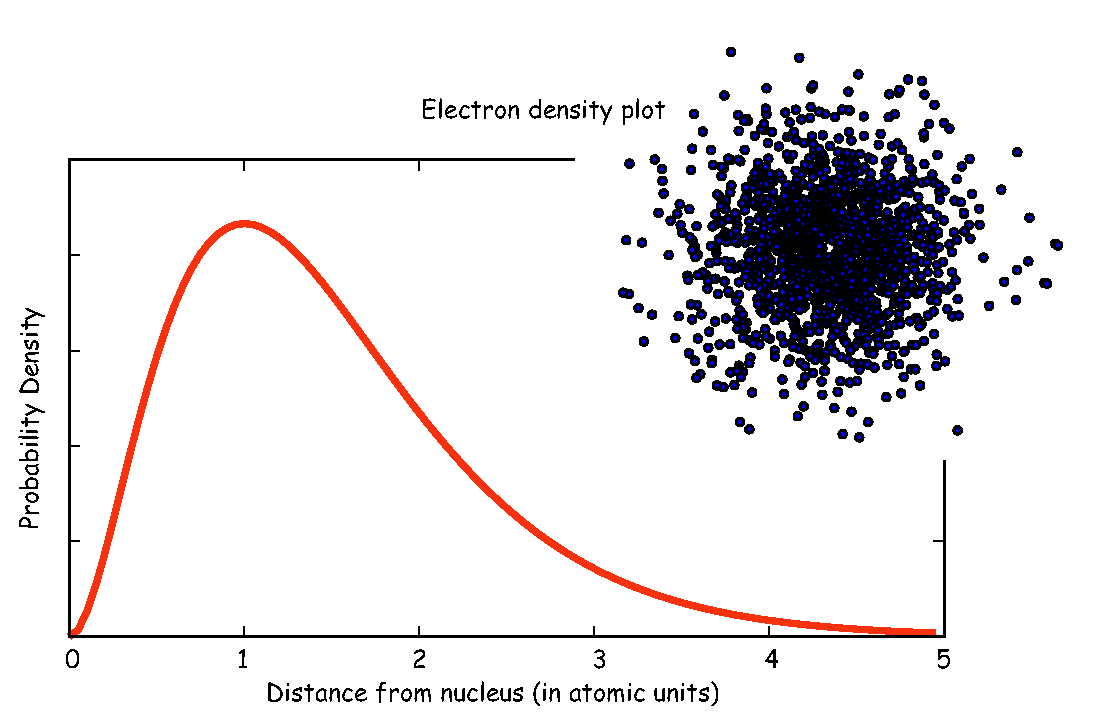
\includegraphics[width=10 cm]{EPSfiles/1s.eps}
\caption{Plot of radial distribution and ``dot-density'' for the 1s electron shell.}
\label{fig:1s}
\end{figure}

\noindent 
 Apparently, this  does not happen, so the classical approach is fatally flawed and we must turn to quantum mechanics.   


\index{quantum!mechanics}
In quantum mechanics,  electronic motion is stabilized  by the fact that electrons can only have certain energy states; they are quantized.   The energy of a given electron can be  described in terms of solutions, $\Psi$, to  something called  
\index{Schr\"odinger's wave equation}
Schr\"odinger's 
wave equation. The function $\Psi(r,\theta,\phi)$ gives the probability  of finding an electron at a given position.   [Remember from Chapter  2 that $r,\theta,\phi$ are the three spherical coordinates.]    It depend on three special
\index{quantum!numbers}
{\it quantum numbers} ($n,l,m$):

\beq
\Psi_{r,\theta,\phi} = R_n^l(r) Y_l^m(\phi,\theta),
\label{eq:wave}
\eeq

\noindent The number $n$ is the so-called ``principal'' quantum number. The $R_n^l(r)$ are functions specific to the element in question and the energy state of the electron $n$.  It is evaluated at an   effective radius $r$ in atomic units.  The $Y_l^m$ are a fully normalized complex representation of the spherical harmonics introduced in Section~\ref{sect:igrf}.     
For each level $n$, the  number $l$ ranges from 0 to $n$-1 and  $m$ from $l$ backwards to $-l$.  

 The lowest energy of the quantum wave equations is found by setting  $n$ equal to unity and both $l$ and $m$ to zero.   Under these conditions, the solution to the wave equation is given by:
 $$
R_{1,0} = 2  Z^{3\over 2}  e^{-\rho/2},
$$
\beq
Y_{0,0}=  ({1\over {4\pi}})^{1\over 2}
\eeq
\noindent where $Z$ is the atomic number and $\rho$ is $2Zr/n$.  Note that at this energy level, there is no dependence of $Y$ on $\phi$ or $\theta$.  Substituting these two equations into Equation~\ref{eq:wave} gives  the probability density  $\Psi$ for  an electron as a function of radius of $r$.  This  is sketched as the line in Figure~\ref{fig:1s}.   Another representation of the same idea is shown in the inset, whereby the density of dots at a given radius reflects the probability distribution shown by the solid curve.  The highest dot density is found at a radius of about one atomic unit, tapering off the farther away from the center of the atom.   Because there is no dependence on $\theta$ or $\phi$ the probability distribution  is a spherical 
\index{electronic!shells}
shell.    All the $l,m=0$ shells are spherical and are often referred to as the 1s, 2s, 3s shells, where the numbers are the energy levels $n$.   A surface with equal probability is a sphere and example of one such shell is shown in Figure~\ref{fig:shells}a.  

For $l=1$, $m$ will have values of -1, 0 and 1 and the $Y_l^m(\phi,\theta)$s are given by:

$$
Y_1^{-1}= {1\over2} \sqrt{{3\over {2\pi}}}\sin\theta e^{-i\phi}, \hskip 1em Y_1^{0}= {1\over2} \sqrt{{3\over {\pi}}}\cos\theta,  \hskip 1em  Y_1^{1}= {-1\over2} \sqrt{{3\over {2\pi}}}\sin\theta e^{i\phi}.
$$
\noindent Shells with $l=1$ depend not only on radial distance but also on the angles $\phi$ and $\theta$, so they are not spheres, but more complicated shapes.  A surface of equal probability for one such shell (the $m=1$ shell) is shown in Figure~\ref{fig:shells}b.  Shells with $l=1$ are called the  ``p'' shells.  

As might be expected,  the shells for  $l=2$ are even more complicated that for $l=1$.  These shells are called   ``d'' shells and two examples are shown in Figure~\ref{fig:shells}c and d.    




\begin{figure}[h!tb]
%\epsfxsize 13cm
%\centering \epsffile {EPSfiles/shells.eps}
\centering  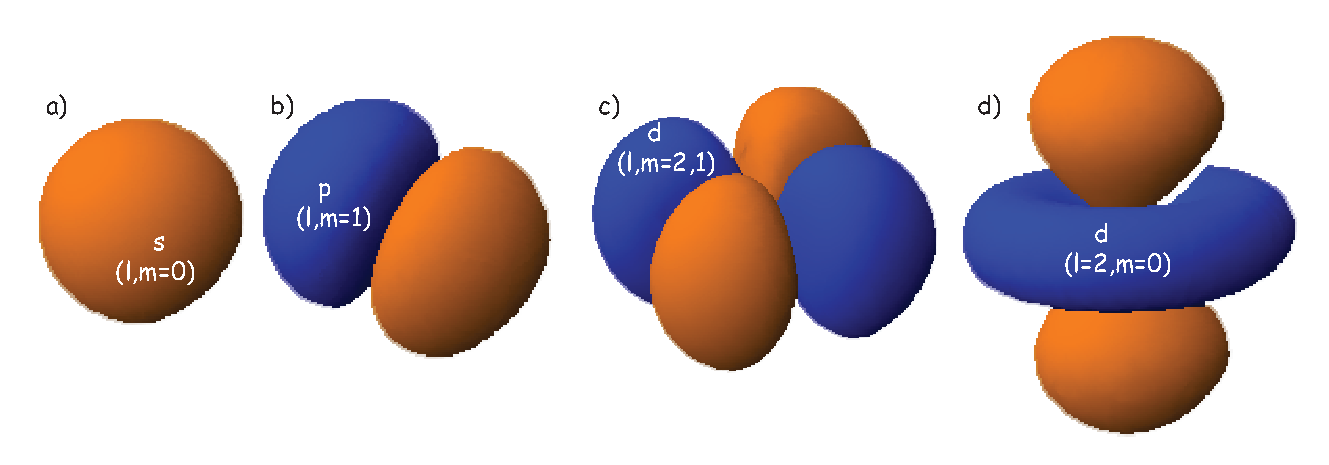
\includegraphics[width=13 cm]{EPSfiles/shells.eps}
\caption{Examples of surfaces of equal probability of the first three shells ($l=1,2,3$).   Surfaces created with Orbital Viewer.    }
\label{fig:shells}
\end{figure}


Returning to the tiny circuit idea,  somehow the motion of the electrons in their shells acts like an electronic circuit and creates a \index{magnetic!moment}
magnetic moment.  
In quantum mechanics,  the angular momentum vector of the electron ${\bf L}$  is quantized, for example as integer multiples of $\hbar$, the 
``reduced'' 
\index{Planck's constant}
Planck's constant (or ${h\over{2\pi}}$ where $h$ = 6.63 x 10$^{-34}$ Js).   The magnetic moment arising from the orbital angular momentum is given by:
$$
|\m| = -{ {q_e}\over {2\mu_e}}|{\bf L}|,
$$
\noindent
where $\mu_e$ is the mass of an electron (9.11 x 10$^{-31}$ kg), $q_e$= -1.69 x 10$^{-19}$C.   The smallest value of ${\bf L}$ is $\hbar$ so 
 the fundamental
unit of magnetic moment arising from the oribit of  electrons is given by:

\beq
|\m_b| = { \hbar 
{q_e}\over {2\mu_e}
} = 9.27 \cross 10^{-24} 
{{\hbox{kg  m}^2}\over {\hbox{s}}}
 \cdot
 {\hbox{C}\over {\hbox{kg}}}
 = 9.27 \cross 10^{-24} {\hbox{Am}^2}.
\label{eq:bohrmagneton}
\eeq

\noindent This is known as  the 
\index{Bohr magneton}
{\it Bohr magneton}.   

\begin{figure}[h!tb]
%\epsfxsize 9cm
%\centering \epsffile{EPSfiles/structure.eps}
\centering  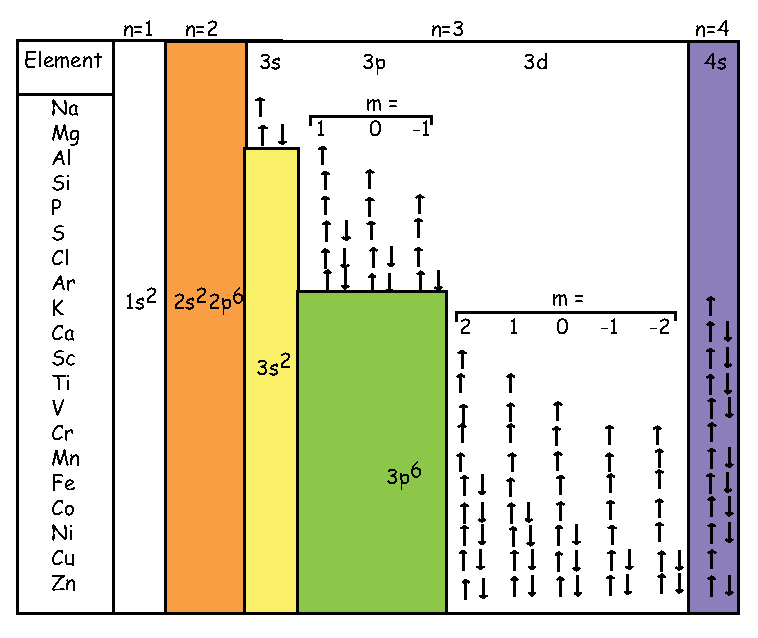
\includegraphics[width=9 cm]{EPSfiles/structure.eps}
\caption{Electronic structure of elements from Na to Zn. }
\label{fig:structure}
\end{figure}


So far we have not mentioned one last quantum number, $s$.  This is the 
\index{electronic!spin}
``spin'' of the electron and has a value of $\pm {1\over 2}$.   The spin itself produces a magnetic moment which is given by $2sm_b$, hence is numerically identical to that produced by the orbit.   

Atoms have the same number of electrons as protons in order to preserve charge balance.  Hydrogen has but one lonely electron which in its lowest energy state sits in the $1s$ electronic shell.  Helium has a happy pair, so where does the second electron go?  To fill in their electronic shells, atoms follow three rules:

\begin{enumerate}

\item No two electrons may have the same set of quantum numbers.  This is 
\index{Pauli's exclusion principle}
Pauli's exclusion principle.  Because spin ($s$) can be $\pm {1\over 2}$, two  electrons fit in one orbital.    When a single electron occupies a given orbital, it is called ``unpaired'' and has a magnetic moment of 1 $m_b$.  

\item Orbitals are filled in order of increasing energy.  The energy state of a given orbital is dependent on the context (whether the atom is bound to other atoms or not), but in general they will be filled according to the scheme shown in Figure~\ref{fig:structure}.  

\item Electrons are added so that the  spins remain as parallel as possible 
\index{Hund's rule}
(Hund's rule).   Notice in  Figure~\ref{fig:structure} that when filling the third energy level ($n=3$), all five $d$ shells  are filled with one kind of spin (say, all up, or +$1\over 2$), before the electrons begin to pair up.  Also, because the energies of the shells change somewhat according to the context they are in, the 4$s$ shell will actually give up an electron to a $d$ shell, before the $d$ shells begin to pair up.    Hund's rule gives the atoms with some $d$ shell electrons (the so-called ``transition elements'', e.g.,  Cr, Mn, Fe, Co and Ni)  the possibility of large magnetic moments.    

\end{enumerate}


Each unpaired spin has a moment of one 
\index{Bohr magneton}
Bohr magneton $m_b$. 
  The elements with the most unpaired spins are the transition elements which  are responsible for 
most of the paramagnetic behavior observed in rocks.     For example, in  Figure~\ref{fig:structure} we see that Mn has a structure of: ($1s^22s^22p^63s^23p^6) 3d^54s^2$, hence has five unpaired spins and a net moment of 5 $m_b$.   Fe  has a structure of ($1s^22s^22p^63s^23p^6) 3d^6 4s^2$ with a net moment of 4 $m_b$,  In minerals, the transition elements are in a variety of oxidation states.  Fe commonly occurs as Fe$^{2+}$ and Fe$^{3+}$.  When losing electrons to form ions, transition metals lose the 4s electrons first, so we have for example, Fe$^{3+}$ with a structure of ($1s^22s^22p^63s^23p^6) 3d^5$, or 5 $m_b$.  Similarly Fe$^{2+}$ has 4 $m_b$ and Ti$^{4+}$ has no unpaired spins.  Iron is the main magnetic species in geological materials, but Mn$^{2+}$ (5 $m_b$) and Cr$^{3+}$ (3 $m_b$) occur in trace amounts.  




\section{Induced magnetization}  

\index{magnetization!induced}
\index{induced magnetization}

We have learned that there are two sources of magnetic moments in electronic motions:  the orbits and the (unpaired)  spins.      These moments respond to external magnetic fields giving rise to an induced magnetization, a phenomenon alluded to briefly in Chapter 1.  We will consider first the contribution of the 
\index{electronic!orbit}
electronic orbits. 

\begin{figure}[htb]
%\epsfxsize 2in
%\centering \epsffile{EPSfiles/larmor.eps}
\centering  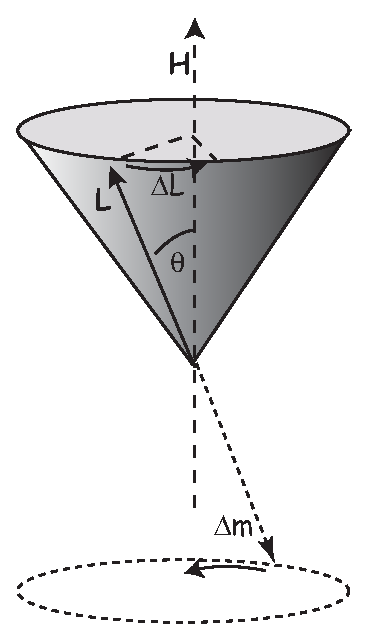
\includegraphics[width=2 in]{EPSfiles/larmor.eps}
\caption{Larmor precession.  The orbit of the electron has an angular momentum vector ${\bf L}$ which creates a magnetic moment.  In the presence of a magnetic field $\H$, the moment experiences a torque which causes a change in angular momentum $\Delta L$.  The precession of the electronic orbit about $\H$ creates an induced magnetic moment $\Delta m$ in a sense opposite to the applied field $\H$.}
\label{fig:larmor}
\end{figure}

\subsection{Orbital contribution and diamagnetism}
\label{sect:dia}


The   angular momentum of  electrons is quantized  in magnitude but also has direction (see  ${\bf L}$ in Figure~\ref{fig:larmor}).  The angular momentum  vector has an associated magnetic moment vector $\m_b$.  A magnetic field $\H$ exerts  a torque on the moment, which nudges it (and the momentum vector associated with it)  to the side ($\Delta L$).  ${\bf L}$  therefore will  precess around the magnetic field direction, much like a spinning top precesses around the direction of gravity.  The precession of ${\bf L}$ is called 
\index{Larmor precession}
{\it Larmor precession}.  

 The changed momentum vector from Larmor precession  in turn results in a   changed
magnetic moment vector $\Delta m$.   The sense of the change in net moment is always to oppose the applied field.
Therefore, the response of  the magnetic moments of electronic orbitals creates an induced magnetization $\M_I$ that is observable outside
the substance;  it is related to the applied field by: 

$$
\M_I=\chi_d \H.
$$

\noindent 
We learned in Chapter 1 that the proportionality between induced magnetization and the applied field    is known as the  
\index{magnetic!susceptibility}%
{\it magnetic susceptibility}.
The ratio $\M_I/\H $ for the response of the electronic orbitals is  termed the 
\index{magnetic!susceptibility!diamagnetic}
\index{diamagnetism}
{\it diamagnetic susceptibility\/} $\chi_d$;  it is negative, 
essentially temperature independent and quite small. This diamagnetic
response is a property of all matter, but for substances whose atoms possess atomic magnetic moments,
diamagnetism is swamped by effects of magnetic fields on the atomic magnetic moments.
  In the absence of unpaired electronic spins, diamagnetic susceptibility dominates the  magnetic response.  Common diamagnetic substances include quartz (SiO$_2$), calcite (CaCO$_3$) and water (H$_2$O).   The mass normalized susceptibility of  quartz is -0.62 x 10$^{-9}$ m$^3$kg$^{-1}$ to give you an idea of the magnitudes of  these things. 

\begin{figure}[htb]
%\epsfxsize 13.5cm
%\centering \epsffile{EPSfiles/para.eps}
\centering  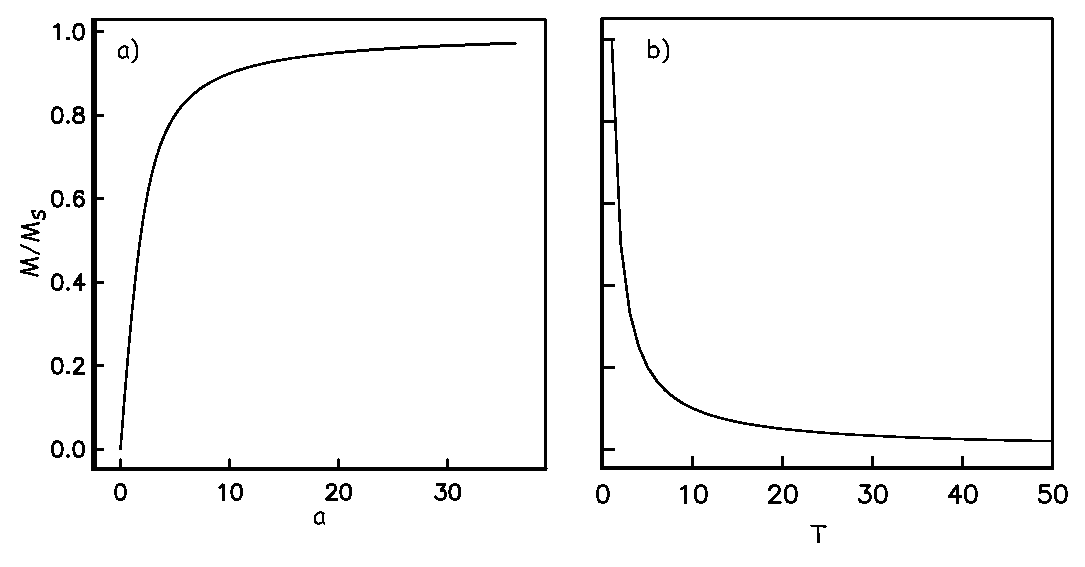
\includegraphics[width=13.5 cm]{EPSfiles/para.eps}
\caption{a) Paramagnetic magnetization (obtained from the Langevin function $\mathcal{L}(a)$ versus $a= mB/kT$.)  b) Paramagnetic magnetization as a function of temperature (Curie Law).}
\label{fig:para}
\end{figure}


\subsection {Role of electronic spins and paramagnetism}
\label{sect:para}

In many geological materials, the orbital contributions cancel out because they are randomly oriented with respect to one another and the magnetization arises from the electronic spins.    We mentioned that unpaired electronic spins  behave as magnetic dipoles with a moment of one 
\index{Bohr magneton}
Bohr magneton. 
In the absence of an applied field, or in  the absence of the  
ordering influence of neighboring
spins which are known as 
\index{exchange!interactions}%
{\it exchange interactions}, the electronic spins are essentially randomly oriented. 
An applied field acts to align the
spins which creates a net magnetization equal to $\chi_p H$ where  
\index{paramagnetism}%
\index{magnetic!susceptibility!paramagnetic}
$\chi_p$ is the {\it paramagnetic susceptibility}.  For
any geologically relevant conditions, the induced magnetization is linearly dependent on the applied field. In paramagnetic solids, atomic magnetic moments react independently to applied magnetic fields and to
thermal energy. At any temperature above absolute zero, thermal energy vibrates the crystal lattice, causing
atomic magnetic moments to oscillate rapidly in random in orientations. In the absence of an applied
magnetic field, atomic moments are equally distributed in all directions with  a resultant magnetization of zero.


A useful first order model for  paramagnetism was worked out by 
\index{Langevin!theory}
P. Langevin in 1905.   (Of course in messy reality things are a bit more complicated, but Langevin theory will work well enough for us at this stage.)
Langevin theory is based on a few simple
premises:


\begin{enumerate}

\item Each unpaired spin contributes a dipole moment. 

\item In the absence of an applied
field, the moments are essentially randomly oriented, \ie
all directions are equally likely to occur.

\item Application of a magnetic field exerts an aligning torque  on the atomic magnetic moments.  The 
\index{magnetic!energy}
magnetic energy $E_m$ (see also Section~\ref{sect:Me} in Chapter 1)  of a 
\index{magnetic!moment}
magnetic moment $\m$ at an angle $\theta$ with an external magnetic
 field $\B=\mu_o \H$ is given by:


\beq
E_m = -\m \cdot \B = -mB  \cos \theta.
\label{eq:Em}
\eeq



 Magnetic energy is at a minimum when the
magnetic moment is lined up with the magnetic field.  

\item There is  competition between the 
\index{magnetic!energy}
magnetic energy $E_m$ and the 
\index{energy!thermal}
 thermal energy $kT$ 
 where $k$ is 
\index{Boltzmann's!constant}
Boltzmann's constant (1.38 x 10$^{-23}$ m$^2$ kg s$^{-2}$ K$^{-1}$) and $T$ is
temperature in kelvin).
\end{enumerate}

Consider an atomic magnetic moment, ($m$ = 2$m_b$ = 1.85$\cross 10^{-23}$
Am$^2$), in a magnetic field of 10$^{-2}$ T, (for reference, the largest  geomagnetic field at the surface is about 65 $\mu$T -- see Chapter 2). The aligning energy is therefore 
$mB$ = 1.85 $\cross$ 10$^{-25}$ J). However, thermal energy at 300K
(traditionally chosen as a temperature close to room temperature providing easy arithmetic) is 
Boltzmann's constant  times the temperature,  or  about  4 x 10$^{-21}$ J.   So thermal energy is several orders of magnitude larger than the
aligning energy and  the net magnetization is small even in this rather large (compared to the Earth's field) magnetizing field.




Using the principles of 
\index{statistical mechanics}
statistical mechanics, we find that the
probability  density of a particular magnetic moment having a 
\index{magnetic!energy}
magnetic energy of  $E_m$ is given by:

\beq
P(E) \propto \exp (-E_m/kT).
\label{eq:PE}
\eeq

\noindent From this we see that the degree of alignment depends exponentially on the ratio of magnetic energy to thermal energy.  The degree of alignment with the magnetic field controls the net magnetization $M$.  When spins are completely aligned, the substance has a
\index{magnetization!saturation}
 {\it saturation magnetization} $M_s$.  The probability density function leads directly to the following relation (derived in  Appendix~\ref{app:langevin}): 

\beq
{M\over {M_s}} =
{ [\hbox{coth }a -
{
1\over{a}
}]=\mathcal{L}(a).
}
\label{eq:Lang} 
\eeq

\noindent where  $a=mB/kT$. The function enclosed in square brackets is known as the 
\index{Langevin!function}
{\it Langevin function} ($\mathcal{L}$).


Equation~\ref{eq:Lang} is plotted in   Figure~\ref{fig:para}a and predicts several intuitive results: 1) $M = 0$ when $B=0$ and 2) $M/M_s = 1$ when the applied  magnetic field is infinite. Furthermore,   $M$  is some 90\% 
of $M_s$ when $mB$ is some 10-20 times $kT$. 
When $kT>> mB, \mathcal{L}(a)$ is approximately linear with a slope of
$\sim 1/3$.  At room temperature and fields up to many tesla, 
$\mathcal{L}(a)$ is approximately $ mB/3kT$. 
\index{paramagnetic susceptibility!low-field}%
If the moments  are unpaired spins ($m=m_b$), then the maximum magnetization possible ($M_s$) is given by the number of moments $N$,  their magnitude ($m_b$) normalized by the volume of the material $v$ or  $M_s=Nm_b/v$,
and

$$
{M\over{M_s}} \simeq {
{ m_b \mu_o }\over
{3kT}
}
H .
$$

Please note that we have neglected all deviations from isotropy including quantum
mechanical effects as well as crystal shape, lattice defects, and state
of stress. These complicate things a little, but to first order the treatment followed here provides  a good approximation.  
We can rewrite the above equation as:


\beq
{M\over H} = {{m_b\mu_o}\over {3kT}}\cdot M_s =
{{Nm_b^2\mu_o}\over{3kv}}\cdot {1\over T} = \chi_p.
\eeq

 To first order,
 paramagnetic susceptibility $\chi_p$ is positive, 
larger than diamagnetism and inversely proportional to temperature.
This inverse T dependence (see Figure~\ref{fig:para}b)  is known as 
\index{Curie's Law}
Curie's law of
paramagnetism.  The paramagnetic susceptibility of, for example, biotite is 790 x 10$^{-9}$ m$^3$ kg$^{-1}$, or about three orders of magnitude larger than quartz (and of the opposite sign!).  


We have considered the simplest case here in which  $\chi$ can be treated as 
a scalar and is referred to as  the
\index{magnetic!susceptibility!bulk}%
{\it bulk magnetic susceptibility} $\chi_b$.
In detail, magnetic susceptibility can be quite complicated. 
The relationship
between induced magnetization and applied field can be
affected by crystal shape, lattice
structure, dislocation density, state of stress, etc., 
which give rise to possible anisotropy of the susceptibility.
Furthermore, there are only a finite number of electronic moments within
a given volume.  When these are fully aligned, the magnetization reaches
saturation.  Thus, magnetic susceptibility is both anisotropic and non-linear
with applied field.

\begin{figure}[htb]
%\epsfxsize 10cm
%\centering \epsffile{EPSfiles/exchange.eps}
\centering  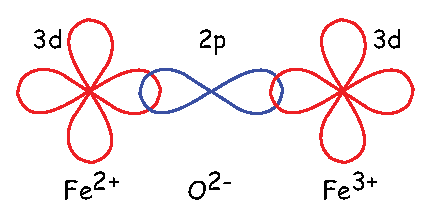
\includegraphics[width=10 cm]{EPSfiles/exchange.eps}
\caption{ Exchange energy associated with overlapping orbitals.  Example of super-exchange between the $3d$ orbitals of two iron cations through the $2p$ orbitals of the intervening oxygen anion.  The  two electrons in the $2p$ shells are, by necessity antiparallel.  These are shared by the $3d$ shells, hence the two cations have anti-parallel spins. [Figure redrawn from O'Reilly, 1984.]}
\label{fig:exchange}
\end{figure}


\section {Ferromagnetism}
\label{sect:ferro}

Some substances give rise to a magnetic field in the absence of an applied field. 
This magnetization  is called {\it remanent } or
\index{magnetization!spontaneous}%
 {\it spontaneous} magnetization, also   loosely known as
\index{ferromagnetism}%
{\it ferromagnetism (sensu lato)}. 
 Magnetic remanence is caused by
strong interactions between neighboring spins that occur in certain
crystals.  

The so-called
\index{exchange!energy}%
{\it exchange energy} is minimized when the spins
are aligned parallel or anti-parallel depending on the details of the crystal
structure.  
Exchange energy is a consequence of the Pauli exclusion principle (no two electrons can have the same set of quantum numbers).  
In the transition elements, the $3d$ orbital is particularly 
susceptible to exchange interactions because of
its shape and the prevalence of unpaired spins, 
 so remanence is characteristic of
certain crystals containing transition elements with unfilled {$ 3d$} orbitals.  

In oxides, oxygen can form a bridge between neighboring cations which are otherwise too far apart for direct overlap of the $3d$ orbitals in a phenomenon known as superexchange.  In Figure~\ref{fig:exchange} the $2p$ electrons of the oxygen are shared with the neighboring $3d$ shells of the iron ions.  Pauli's exclusion principle means that the shared electrons must be antiparallel to each of  the electrons in the $3d$ shells.  The result is that the two cations are coupled.  In the case shown in Figure~\ref{fig:exchange} there is an Fe$^{2+}$ ion coupled antiparallel to an Fe$^{3+}$ ion.  For two ions with the same charge, the coupling will be parallel.  Exchange energies are huge, equivalent to the energy associated with the same moment in  a field of the order of 1000 T.  [The largest field available in the Scripps paleomagnetic laboratory is about 2.5 T, and that only fleetingly.]
 

 
As temperature increases,  crystals expand and exchange  becomes weaker.
 Above a temperature characteristic of
 each crystal type (known as the
 \index{Curie temperature}
  {\it Curie temperature}
 $T_c$), cooperative spin  behavior disappears entirely and the material becomes 
paramagnetic.  

 
\begin{figure}[htb]
%\epsfxsize 12cm
%\centering \epsffile{EPSfiles/MsT.eps}
\centering  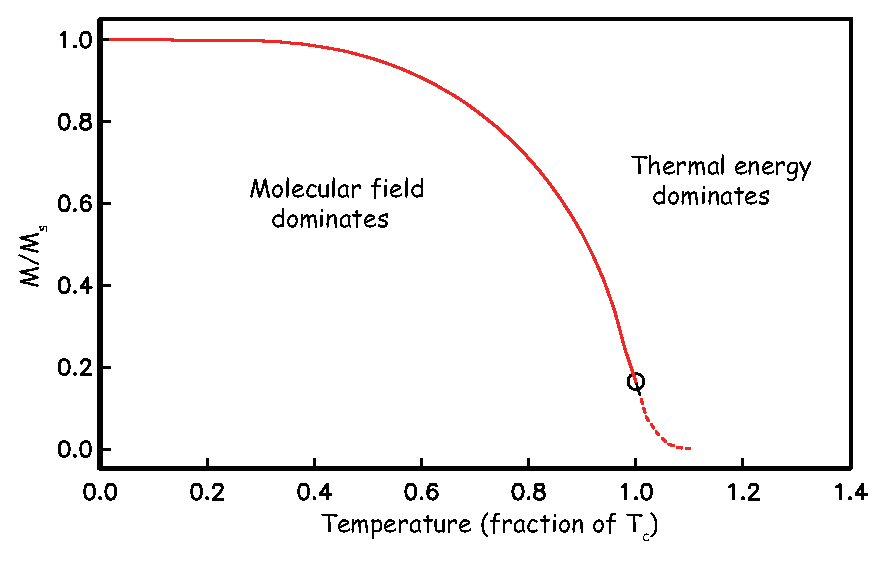
\includegraphics[width=12 cm]{EPSfiles/MsT.eps}
\caption{Behavior of magnetization versus temperature of a ferromagnetic
substance.  Below $T_c$, the magnetization follows Equation 3.9 and is the ferromagnetic magnetization.  Above $T_c$  the magnetization follows Equation 3.8 and is the induced magnetization. [Redrawn from Tauxe, 1998.]  }
\label{fig:MsT}
\end{figure}
\nocite{tauxe98}

While the phenomenon of ferromagnetism results from complicated
interactions of neighboring spins, it is useful to think of the
ferromagnetic moment as resulting from a quasi-paramagnetic response to
a huge internal field.  This imaginary field is termed the 
\index{Weiss molecular field}
{\it Weiss molecular field} $H_w$.  In 
Weiss theory, $H_w$ is proportional to the
magnetization of the substance, i.e., 

$$
H_w = \beta M,
$$

\noindent
where $\beta$ is the constant of proportionality.
The total magnetic field that the substance experiences is:

$$
H_{tot} = H + H_w = H + \beta M,
$$

\noindent where $H$ is the external field.  By analogy to paramagnetism,
we can substitute $a=\mu_om_b(H_{tot})/kT)$ for $H$ in
\index{Langevin!function}
 Langevin function:

\beq
{M  \over {M_s}} {= \mathcal{L} \left({ {\mu_o m_b(H+\beta M)}\over{kT} } \right)}.
\label{eq:Mweiss}
\eeq

\noindent For temperatures above the Curie temperature $T_c$ (i.e.
$T-T_c>0$) there is by definition no internal field, hence  $\beta M$  is zero.
Substituting $N m_b/v$ for $M_s$, and using the low-field approximation
for $\mathcal{L} (a)$, Equation~\ref{eq:Mweiss} can 
be rearranged to get:

\index{Curie-Weiss law}%
\beq
{M\over H} = { {\mu_o N m_b^2}\over {v3k(T-T_c)} } \equiv \chi_f.
\label{eq:curieweiss}
\eeq

\noindent
Equation~\ref{eq:curieweiss} is known as the Curie-Weiss law and governs
ferromagnetic susceptibility above the Curie temperature (dashed line in Figure~\ref{fig:MsT}). 

\begin{figure}[htb]
%\epsfxsize 11cm
%\centering \epsffile{EPSfiles/curie.eps}
\centering  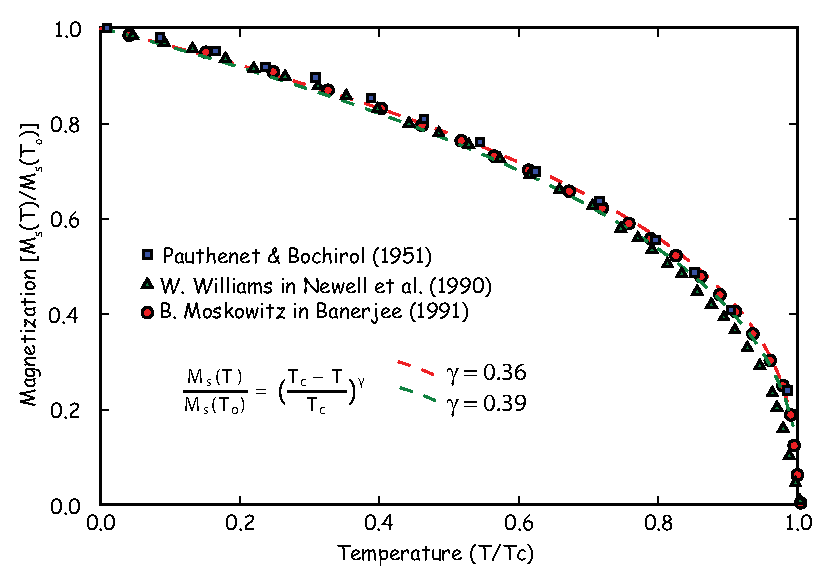
\includegraphics[width=11 cm]{EPSfiles/curie.eps}
\caption{Various data sets for  the behavior of $M_s(T)$ for magnetite.     }
\label{fig:curie}
\end{figure}
\nocite{pauthenet51,newell90,banerjee91}

Below the Curie temperature $H_w>>H$;  we can neglect the external field $H$  and 
get:


$$
{M\over {M_s}} = \mathcal{L}  \bigl( {{\mu_o m_b \beta M}\over{kT}}\bigr).
$$ 

\noindent Substituting again for $M_s$ and rearranging, we get:


\beq
{M\over M_s} = \mathcal{L} \bigl( {{Nm_b^2 \beta}\over{vkT}}\cdot {M\over M_s}
\bigr) =
\mathcal{L}  \bigl( {T_c \over T} \cdot {M\over M_s} \bigr),
\label{eq:Mferro}
\eeq
\index{Curie temperature}%
\noindent where $T_c$ is the Curie temperature and is given by:
$$T_c = { {Nm_b^2 \beta}\over{vk}}.$$
\noindent  
Equation~\ref{eq:Mferro} can be solved graphically or
numerically and is sketched (solid line)  in Figure~\ref{fig:MsT}.  Below the Curie
temperature, exchange interactions are strong relative to the
external field and  the magnetization is
governed by Equation~\ref{eq:Mferro}. Above the Curie temperature, it
follows the Curie-Weiss law (Equation~\ref{eq:curieweiss}).  




We have treated ferromagnetism from a classical point of view and this is strictly incorrect because ferromagnetism  results primarily from quantum mechanical phenomena.  The primary difference  between the classical derivation and the quantum mechanical one lies in the fact that in quantum mechanics, only certain angles of the magnetic moments are allowed, as opposed to all directions in Langevin theory.  In the end, the predictions of magnetization as a function of temperature are different in detail.   The end product of the quantum mechanical treatment 
\index{Dunlop, D.J.}
\index{\"Ozdemir, \"O.}
(see Dunlop and \"Ozdemir, 1997) \nocite{dunlop97} is that the variation of 
\index{magnetization!saturation}
saturation magnetization as a function of temperature can be reasonably well approximated (near the
\index{Curie temperature}
 Curie Temperature, $T_c$) by a normalized power law variation:
\begin{equation}
{M_s(T)\over {M_s(T_o)}} = \bigl[{  {T_c - T}\over{T_c-T_o}} \bigr]^{\gamma },
\label{eq:MsT}
\end{equation}

\noindent  where  $\gamma$ is 0.5 from simple molecular field theory and $T_o$ is absolute zero (in kelvin).   Dunlop and \"Ozdemir (1997) cite a value of around 0.43 for $\gamma$, but the  data sets cited by Dunlop and \"Ozdemir (1997; e.g., Figure 3.5 on page 52) are actually best-fit with values for $\gamma$ of about 0.36 -- 0.39 (see Figure~\ref{fig:curie}).   These curves have been normalized by their inferred curie Temperatures which are around 565$^{\circ}$C (data of B. Moskowitz, cited in
\index{Banerjee, S.K.}
 Banerjee, 1991).  \nocite{banerjee91} 

\begin{figure}[h!tb]
%\epsfxsize 14cm
%\centering \epsffile{EPSfiles/spins.eps}
\centering  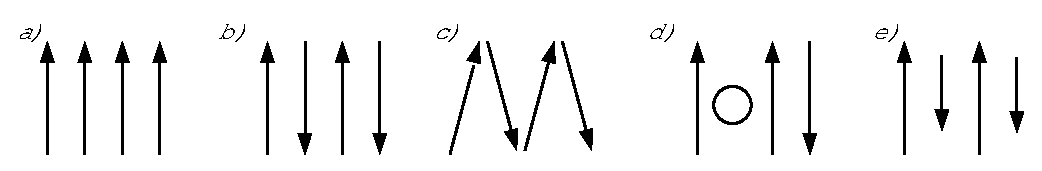
\includegraphics[width=14 cm]{EPSfiles/spins.eps}
\caption{Types of spin alignment in ferromagnetism {\it (sensu lato)}:
a) ferromagnetism ({\it sensu stricto}), b) antiferromagnetism, c)
spin-canted antiferromagnetism, d) defect anti-ferromagnetism, e)
ferrimagnetism.
}
\label{fig:spins}
\end{figure}



\index{ferromagnetism}%

As we have seen,
below the Curie temperature, certain crystals have a permanent
(remanent) magnetization resulting from the alignment of unpaired
electronic spins over a large area within the crystal.  Spins may be
 either parallel or anti-parallel;
the sense of spin alignment is controlled
entirely by crystal structure. The energy term associated with this
phenomenon is the 
\index{exchange!energy}%
{exchange energy}. 
\index{ferromagnetism}%
\index{ferrimagnetism}%
\index{antiferromagnetism}%
 There are three categories of spin alignment: ferromagnetism ({\it
sensu stricto}),  ferrimagnetism and antiferromagnetism (see
Figure~\ref{fig:spins}).  

 \begin{figure}[htb]
 %\epsfxsize 14cm
 %\centering \epsffile{EPSfiles/spinwave.eps}
 \centering  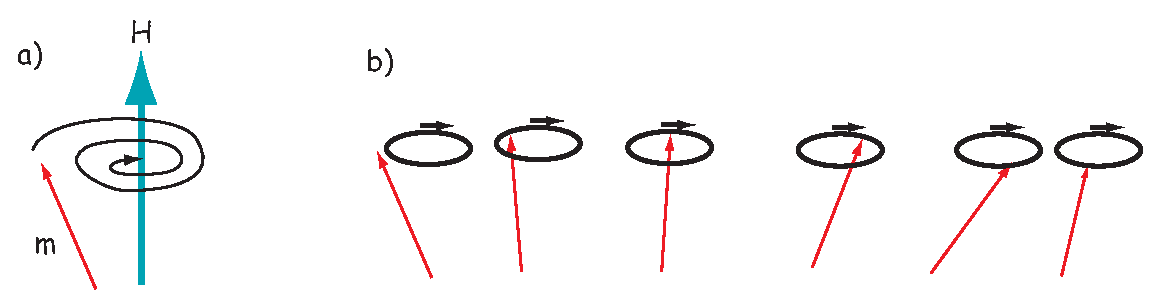
\includegraphics[width=14 cm]{EPSfiles/spinwave.eps}
 \caption{a) Response of a magnetic moment to the torque of an applied field for isolated moments.  b) Response of coupled moments to a perturbation. Neighboring spins produce an effect known as ``spin waves''.}
 \label{fig:spinwave}
 \end{figure}
 


\index{ferromagnetism}%
In {\it ferromagnetism} ({\it sensu stricto}, Figure~\ref{fig:spins}a), the
\index{exchange!energy}%
 exchange energy is minimized when all the spins
are  parallel, as occurs in  pure
\index{iron}%
iron.  When spins are perfectly
antiparallel 
\index{antiferromagnetism}%
({\it antiferromagnetism}, Figure~\ref{fig:spins}b), 
there is no net magnetic moment, as occurs
in 
\index{ilmenite}%
ilmenite.    Occasionally, the antiferromagnetic spins are not 
perfectly aligned in an  antiparallel orientation, but are canted by a 
few degrees.  This
\index{spin-canting}%
{\it spin-canting} (Figure~\ref{fig:spins}c) gives rise to
a weak net moment, as occurs in 
\index{hematite}%
hematite, a common magnetic mineral (see Chapter 6).  Also, antiferromagnetic materials can
have a net moment if spins are not perfectly compensated owing to
defects in the crystal structure, as occurs in fine-grained hematite.
The uncompensated spins result in a so-called {\it
defect} moment (Figure~\ref{fig:spins}d).   
We note in passing that the temperature at which spins become disordered
in antiferromagnetic substances is termed the 
\index{N\'eel!temperature}%
{\it N\'eel temperature}. In
\index{ferrimagnetism}%
 {\it ferrimagnetism},  spins are also aligned antiparallel, but the
magnitudes of the moments in each direction are unequal, resulting
in a net moment (Figure~\ref{fig:spins}e). 


In figures like Figure~\ref{fig:spins},  electronic spins are depicted as being simply aligned with some minimum energy  direction (aligned with the field, or along some easy axis).  Yet we already know about the paramagnetic effect of misalignment through  random thermal fluctuations.   We learned that an external magnetic field generates a torque  on the electronic spins, and in isolation, a magnetic moment will respond to the torque in a manner similar in some respects to  the way a spinning top responds to gravity: the magnetic moment will precess about the applied field direction, spiraling in  and come to a rest parallel to it (Figure~\ref{fig:spinwave}a). Because of the strong exchange coupling  in ferromagnetic phases, spins tend to be aligned parallel (or antiparallel) to one another and the spiralling is done in a coordinated fashion, with neighboring spins as parallel as possible to one another (Figure~\ref{fig:spinwave}b).   This phenomenon is known as a 
\index{spin waves}%
{\it spin wave}.  
 
 
\vskip .5 in\noindent{SUPPLEMENTAL READINGS:} O'Reilly (1984), Chapter 3.1;    \nocite{oreilly84}
Dunlop and \"Ozdemir (1997), Chapter 2.1 to 2.7.

\vskip 24pt
{{\parindent 0pt \parskip 12pt 







\section{Problems }



{\bf Problem 1}

a) Given one Bohr magneton ($m_b$) in the Earth's field (40 $\mu$T), write a program using Python that calcuates magnetostatic interaction energy (-$m_bB\cos \theta$) for angles 0$\rightarrow$ 180$^{\circ}$.   Make a plot of this with the {\bf matplotlib} module in Python.  

b) Calculate the thermal energy at room temperature (300K).     How does this compare with the interaction energy? 

{\bf Problem 2}


Fayalite (Fe$_2$SiO$_4$) is a paramagnetic solid with magnetic susceptibility $\chi$ = 4.4 x 10$^{-4}$ (cgs units) at 0$^{\circ}$C (= 273K).  
A single crystal of fayalite has a volume of 2 cm$^{3}$.  This crystal is placed in a magnetic field, $H=10$ oe at 0$^{\circ}$C.  What is the resulting induced magnetic  moment $m$ of this crystal?  


a)  Do this problem first in cgs units.  Then convert your answer to SI using the conversion factors in Table \ref{tab:units}  in Chapter 1. 

b)  Do the problem again  by first converting all the parameters into SI units.  Check your answer by converting the SI answer that you get back to cgs.  You should get the same answer (but you would be surprised how many people do this wrong).   

{\bf Problem 3}

If fayalite is placed in a magnetic field $H$= 100 oe at a temperature of 500$^{\circ}$C (= 773K), what is the resulting magnetization, $M$?   



{\bf Problem 4}

  MnS is a paramagnetic solid.  At 300K there are 4 x 10$^{28}$ molecules of MnS per m$^3$. Look up the number of unpaired spins for the cationic magnetic moment of Mn$^{2+}$  in the text and find  the paramagnetic susceptibility, $\chi$, of MnS at 300K?

{\bf Problem 5 } 

a) Read into a Pandas DataFrame  the datafile {\it Chapter\_3/BMoskinBan91.txt} provided.   Make a plot of magnetization versus temperature.  
  What is the Curie temperature of the material?
  
 b) Using this Equation~\ref{eq:MsT} from the chapter, find the value for $\gamma$ between 0.35 and 0.43 at intervals of 0.01 that fits the best.    Plot the data as in Figure~\ref{fig:curie} in the chapter, i.e. $M_s(T)/Ms(T_o)$ against $T/T_c$.  



%http://quantlab.bu.edu/acrosby/orbitals/dxy.html
